\documentclass[english]{article}
%%%%%%%%%%%%%%%%%%%%%%%%%%%%%%%%%%%%%%%%%%%%%%%%%%%%%%%%%%%%%%%%%%%%%%%%%%%%%%%%%%%%%%%%%%%%%%%%%%%%%%%%%%%%%%%%%%%%%%%%%%%%
\usepackage{latexsym,amsmath,amssymb,amsfonts,fullpage}
\usepackage{graphicx,float}
% For code listing
\usepackage{listings}
\usepackage{color}
\definecolor{keywords}{RGB}{255,0,90}
\definecolor{comments}{RGB}{0,0,113}
\definecolor{red}{RGB}{160,0,0}
\definecolor{myblack}{RGB}{0,0,0}
\definecolor{mybgcolor}{RGB}{220,220,220}
\definecolor{green}{RGB}{0,150,0}
\lstset{language=Matlab, 
        backgroundcolor=\color{mybgcolor},
        frame=single,
        basicstyle=\ttfamily\small, 
        keywordstyle=\color{keywords},
        commentstyle=\color{comments},
        stringstyle=\color{red},
        showstringspaces=false,
        identifierstyle=\color{myblack}}

\begin{document}
	
\begin{center}
{\textbf{MEAM 620 Homework 2}} \\
Due: February 18, 2015, 11:59pm
\end{center}


\paragraph{1.} List two advantages and two disadvantages each for using (a) rotation matrices;(b) axis angle representation; (c) exponential coordinates; (d) Euler angles; and (e) quaternions to describe rotations? 
\[\textrm{ }\]
\begin{enumerate}
 \item[(a)] Rotation matrices 
    \begin{itemize}
     \item Advantages
     \begin{enumerate}
      \item[1.] Very easy to use in coordinates - just use matrix multiplication with point you want to rotate
      \item[2.] Covers all of $SO(3)$, since rotation matrices are how $SO(3)$ is defined. 
     \end{enumerate}
     \item Disadvantages
     \begin{enumerate}
      \item[1.] Not very compact - only need 3 numbers to represent $SO(3)$, but here we use 9
      \item[2.] Interpolation - interpolating between 2 rotation matrices is non-trival, and we often want to do this.
     \end{enumerate}
    \end{itemize}

 \item[(b)] Axis-Angle Representation 
    \begin{itemize}
     \item Advantages
     \begin{enumerate}
      \item[1.] Compact representation - just need 4 numbers to represent it (3 for axis, 1 for angle). 
      \item[2.] Covers all of $SO(3)$ - every matrix can be represented this way (similar to axis-angle) (with singularities as shown below)
     \end{enumerate}
     \item Disadvantages
     \begin{enumerate}
      \item[1.] Many to one representation - the zero rotation has infinitely many representations,
                and even if you restrict the angle to $[0,pi]$, then you get $R(x,\pi) = R(-x,\pi)$
                (though the latter is an inherent problem in $SO(3)$). 
      \item[2.] More difficult to compute with - need to convert into rotation matrix before you can use
     \end{enumerate}
    \end{itemize}

 \item[(c)] Exponential Coordinates 
    \begin{itemize}
     \item Advantages
     \begin{enumerate}
      \item[1.] Compact representation - just need 3 numbers to represent it (3 for axis times the angle) (Can also represent as axis and angle). 
      \item[2.] Covers all of $SO(3)$ - every matrix can be represented this way (similar to axis-angle), and avoids singularities of axis-angle
     \end{enumerate}
     \item Disadvantages
     \begin{enumerate}
      \item[1.] More difficult to compute with - need to convert into rotation matrix before you can use, like axis-angle
      \item[2.] Many to one map - This still is a many to one representation of $SO(3)$, since we have the $(x,\pi)$ and $(-x,\pi)$
                axis angle singularity.
     \end{enumerate}
    \end{itemize}

 \item[(d)] Euler angles 
    \begin{itemize}
     \item Advantages
     \begin{enumerate}
      \item[1.] Compact representation - just need 3 numbers to represent it, one for each angle.  
      \item[2.] Easy to compute with - just need to compute the 3 rotation matrices to do it (which is comparitively easy)
     \end{enumerate}
     \item Disadvantages
     \begin{enumerate}
      \item[1.] Singularities - Gimbal lock is a big problem if you are dealing with large rotations
      \item[2.] 
     \end{enumerate}
    \end{itemize}

 \item[(e)] Quaternions 
    \begin{itemize}
     \item Advantages
     \begin{enumerate}
      \item[1.] Compact representation - just need 4 numbers to represent it, one for each angle.
      \item[2.] Easy to compute with - It is very fast to compute a rotation with a quaternion - just use $qpq^{-1}$. Also easy to compose quaternions
     \end{enumerate}
     \item Disadvantages
     \begin{enumerate}
      \item[1.] Renormalization - quaternions MUST be of unit length, so you have to renormalize every time you combine quaternions
      \item[2.] 
     \end{enumerate}
    \end{itemize}

\end{enumerate}



\paragraph{2.}  
Consider the problem of fitting a smooth curve to the following waypoints in 2D: 
\begin{align*}
t_0 &= 0, (x_0, y_0) = (-1, 0) \\
t_1 &= 5, (x_1, y_1) = (0, 2) \\
t_2 &= 6, (x_2, y_2) = (1, 0) \\
t_0 &= 0, (\dot{x}_0, \dot{y}_0) = (-1, -5) 
\end{align*}

Note that the first three constraints are position constraints, while the last is a velocity constraint. Any other necessary derivative constraints at $t_0 = 0$ and $t_2 = 6$ should be set to $(0, 0)$. To minimize the functional:
\begin{align}
\int_{t = 0}^T \| x^{(n)} \|^2 dt,
\end{align}

\noindent the endpoints need to be constrained in position, velocity, and up to and including the $(n-1)$st derivative. All derivatives (velocity, acceleration, etc.) at $t_1 = 5$ should be left unspecified, and you will need to add the appropriate number of continuity constraints at that point. Also, note you will need to find $x(t)$ and $y(t)$.

\begin{enumerate}
 \item[a.] A minimum acceleration trajectory can be constructed by fitting a cubic spline. Construct this trajectory for the waypoint constraints above. Explicitly write down the solution you find (ie. write down $x(t) = c_0 + c_1 t + c_2 t^2 ...$, where you fill in $c_0, c_1, c_2, ...$ with the coefficient values you found) and create a plot illustrating each trajectory and the waypoints. Include your Matlab code with your submission. 

As we are using a cubic spline, we need two sets of coefficents to represent this curve, 8 total.
We use the following code to find the coefficents for the cubic spline: 
\begin{lstlisting}
% Create constants for the spline
X    = [ -1;   0;   1 ];
Y    = [  0;   2;   0 ];
Xdot = [ -1; nan; nan ]; % Don't know the last two...
Ydot = [ -5; nan; nan ]; % Don't know the last two...
T    = [  0;   5;   6 ];

A = zeros(8,8); % 8x8 coefficient matrix
bx = zeros(8,1); % The x-direction result vector
by = zeros(8,1); % The y-direction result vector
% Time 1 constraints
A(1,1:4) =  [T(1)^3, T(1)^2, T(1), 1]; % Positions
bx(1)    =  X(1);
by(1)    =  Y(1);
A(2,1:4) =  [3*T(1)^2, 2*T(1), 1, 0]; % Velocities
bx(2)    =  Xdot(1);
by(2)    =  Ydot(1);

% Time 2 constraints
A(3,1:4) =  [T(2)^3, T(2)^2, T(2), 1]; % Final position for first segment
bx(3)    =  X(2);
by(3)    =  Y(2);
A(4,5:8) =  [T(2)^3, T(2)^2, T(2), 1]; % Initial position for second
bx(4)    =  X(2);
by(4)    =  Y(2);
A(5,1:4) =  [3*T(2)^2, 2*T(2), 1, 0]; % Velocities must be the
A(5,5:8) = -[3*T(2)^2, 2*T(2), 1, 0]; %   same for both segments
bx(5)    =  0;
by(5)    =  0;
A(6,1:4) =  [6*T(2), 2, 0, 0]; % Accelerations must be the
A(6,5:8) = -[6*T(2), 2, 0, 0]; %   same for both segments
bx(6)    =  0;
by(6)    =  0;

% Time 3 constraints
A(7,5:8) =  [T(3)^3, T(3)^2, T(3), 1]; % Final position for first segment
bx(7)    =  X(3);
by(7)    =  Y(3);
A(8,5:8) =  [3*T(3)^2, 2*T(3), 1, 0]; % Velocity vanishes at the end
bx(8)    =  0;
by(8)    =  0;

% Compute the coefficents
Cx = A \ bx;
Cy = A \ by;

\end{lstlisting}

This gives us our spline coefficents:
\[ x(t) = \begin{cases}
           (-0.000667)t^3 + (0.243333)t^2 + (-1.000000)t + (-1.000000)  & \textrm{ if } 0 \leq t \leq 5 \\
           (-0.616667)t^3 + (9.483333)t^2 + (-47.200000)t + (76.000000) & \textrm{ if } 5 \leq t \leq 6 \\
          \end{cases} \]
\[ y(t) = \begin{cases}
           (-0.311333)t^3 + (2.636667)t^2 + (-5.000000)t + (0.000000)      & \textrm{ if } 0 \leq t \leq 5 \\
           (2.016667)t^3 + (-32.283333)t^2 + (169.600000)t + (-291.000000) & \textrm{ if } 5 \leq t \leq 6 \\
          \end{cases} \]

The plot looks as follows:
\begin{figure}[H]
\centering
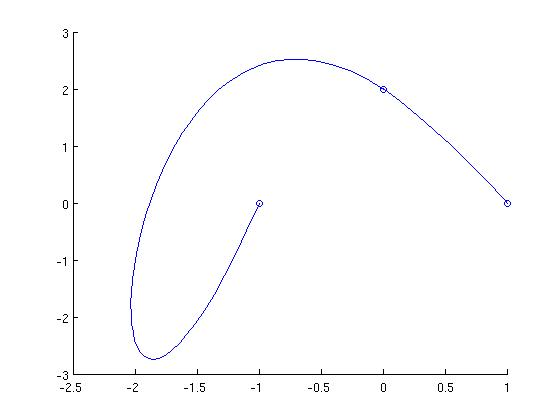
\includegraphics[scale=0.5]{cubicspline.jpg}
\caption{The plot of the cubic spline}
\end{figure}

\item[b.] What is the minimum order polynomial you need to construct a minimum jerk trajectory? Construct this trajectory, write down your solution, and create a plot as in part a. 

As shown in class, using the Euler-Lagrange equations, it is a quintic polynomial, or one of order 6 (highest degree 5). So we compute it as follows:
\begin{lstlisting}
% Create constants for the spline
X    = [ -1;   0;   1 ];
Y    = [  0;   2;   0 ];
Xdot = [ -1; nan; nan ]; % Don't know the last two...
Ydot = [ -5; nan; nan ]; % Don't know the last two...
T    = [  0;   5;   6 ];

A = zeros(12,12); % 12x12 coefficient matrix
bx = zeros(12,1); % The x-direction result vector
by = zeros(12,1); % The y-direction result vector
seg1 = 1:6;
seg2 = 7:12;
% Time 1 constraints
% Initial positions
A(1,seg1)  =  [T(1)^5, T(1)^4, T(1)^3, T(1)^2, T(1), 1]; 
bx(1)      =  X(1);
by(1)      =  Y(1);
% Initial velocity
A(2,seg1)  =  [5*T(1)^4 4*T(1)^3 3*T(1)^2 2*T(1) 1 0];
bx(2)      =  Xdot(1);
by(2)      =  Ydot(1);
% Initial acceleration
A(3,seg1)  =  [20*T(1)^3 12*T(1)^2 6*T(1) 2 0 0];
bx(3)      =  0;
by(3)      =  0;

% Time 2 constraints
% Final position for first segment
A(4,seg1)  =  [T(2)^5, T(2)^4, T(2)^3, T(2)^2, T(2), 1];
bx(4)      =  X(2);
by(4)      =  Y(2);
% Initial position for second
A(5,seg2)  =  [T(2)^5, T(2)^4, T(2)^3, T(2)^2, T(2), 1];
bx(5)      =  X(2);
by(5)      =  Y(2);
% Velocities must be the same for both segments
A(6,seg1)  =  [5*T(2)^4 4*T(2)^3 3*T(2)^2 2*T(2) 1 0];
A(6,seg2)  = -[5*T(2)^4 4*T(2)^3 3*T(2)^2 2*T(2) 1 0];
bx(6)      =  0;
by(6)      =  0;
% Accelerations must be the same for both segments
A(7,seg1)  =  [20*T(2)^3 12*T(2)^2 6*T(2) 2 0 0];
A(7,seg2)  = -[20*T(2)^3 12*T(2)^2 6*T(2) 2 0 0];
bx(7)      =  0;
by(7)      =  0;
% Jerk must be the same for both segments
A(8,seg1)  =  [60*T(2)^2 24*T(2) 6 0 0 0];
A(8,seg2)  = -[60*T(2)^2 24*T(2) 6 0 0 0];
bx(8)      =  0;
by(8)      =  0;
% Snap must be the same for both segments
A(9,seg1)  =  [120*T(2) 24 0 0 0 0];
A(9,seg2)  = -[120*T(2) 24 0 0 0 0];
bx(9)      =  0;
by(9)      =  0;

% Time 3 constraints
% Final position for first segment
A(10,seg2) =  [T(3)^5, T(3)^4, T(3)^3, T(3)^2, T(3), 1];
bx(10)     =  X(3);
by(10)     =  Y(3);
% Velocity vanishes at the end
A(11,seg2) =  [5*T(3)^4 4*T(3)^3 3*T(3)^2 2*T(3) 1 0];
bx(11)     =  0;
by(11)     =  0;
% Final acceleration
A(12,seg2) =  [20*T(3)^3 12*T(3)^2 6*T(3) 2 0 0];
bx(12)     =  0;
by(12)     =  0;

% Compute the coefficents
Cx = A \ bx;
Cy = A \ by;

\end{lstlisting}

This gives us our spline coefficents (this time only up to 4 decimal places due to their length):

\(x(t) = \)
\[
\begin{cases}
(-0.0086)t^5 + (0.0823)t^4 + (-0.1478)t^3 + (0)t^2 + (-1)t + (-1) & \textrm{ if } 0 \leq t \leq 5 \\
(0.3431)t^5 + (-8.7097)t^4 + (87.7722)t^3 + (-439.6)t^2 + (1098)t + (-1100) & \textrm{ if } 5 \leq t \leq 6 \\
\end{cases}
\]

\(y(t) = \)
\[
\begin{cases}
(0.0470)t^5 + (-0.5892)t^4 + (1.9878)t^3 + (0)t^2 + (-5)t + (0) & \textrm{ if } 0 \leq t \leq 5 \\
(-0.9505)t^5 + (24.3468)t^4 + (-247.3722)t^3 + (1246.8)t^2 + (-3122)t + (3117) & \textrm{ if } 5 \leq t \leq 6 \\
\end{cases}
\]

%\[ x(t) = \begin{cases}
%           (-0.0086)t^5 + (0.0822)t^4 + (-0.1477)t^3 + (0)t^2 + (-1)t + (-1)         & \textrm{ if } 0 \leq t \leq 5 \\
%           (0.3430)t^5 + (-8.7097)t^4 + (87.7722)t^3 + (-439.6)t^2 + (1098)t + (-1100) & \textrm{ if } 5 \leq t \leq 6 \\
%          \end{cases} \]
%\[ y(t) = \begin{cases}
%           (0.0469)t^5 + (-0.5892)t^4 + (1.9877)t^3 + (0)t^2 + (-5)t + (0) & \textrm{ if } 0 \leq t \leq 5 \\
%           (-0.9504)t^5 + (24.3467)t^4 + (-247.3722)t^3 + (1246.8)t^2 + (-3122)t + (3117) & \textrm{ if } 5 \leq t \leq 6 \\
%          \end{cases} \]

The plot looks as follows:
\begin{figure}[H]
\centering
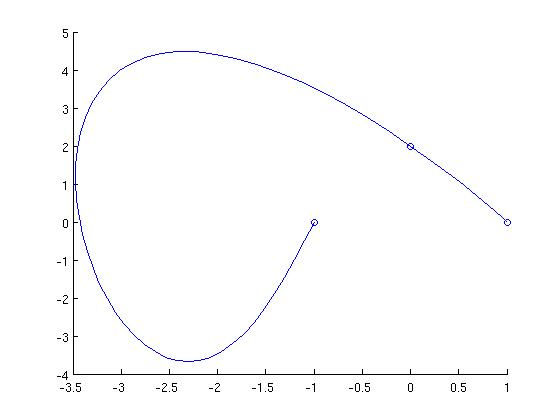
\includegraphics[scale=0.5]{quinticspline.jpg}
\caption{The plot of the quintic spline}
\end{figure}

\item[c.] What is the minimum order polynomial you need to construct a minimum snap trajectory? Construct this trajectory, write down your solution, and create a plot. 
We use the Euler-Lagrange equations to determine what degree you need:
\[ \mathcal{L} = (x^{(4)})^2 \]
\[ \frac{\partial \mathcal{L}}{\partial x} - \frac{d}{dt} \left( \frac{\partial \mathcal{L}}{\partial \dot{x}} \right)
  - \frac{d^2}{dt^2} \left( \frac{\partial \mathcal{L}}{\partial \ddot{x}} \right)
  - \frac{d^3}{dt^3} \left( \frac{\partial \mathcal{L}}{\partial x^{(3)}} \right)
  - \frac{d^4}{dt^4} \left( \frac{\partial \mathcal{L}}{\partial x^{(4)}} \right)
  =  - \frac{d^4}{dt^4} \left( 2 x^{(4)} \right) = -2 x^{(8)} = 0\]
  \[ \implies x^{(8)} = 0 \]
  
  So we need a polynomial of order 8, or dergree 7. We again compute as follows:

\begin{lstlisting}
% Create constants for the spline
X    = [ -1;   0;   1 ];
Y    = [  0;   2;   0 ];
Xdot = [ -1; nan; nan ]; % Don't know the last two...
Ydot = [ -5; nan; nan ]; % Don't know the last two...
T    = [  0;   5;   6 ];

A = zeros(16,16); % 16x16 coefficient matrix
bx = zeros(16,1); % The x-direction result vector
by = zeros(16,1); % The y-direction result vector
seg1 = 1:8;
seg2 = 9:16;
% Time 1 constraints
% Initial positions
A(1,seg1)  =  [T(1)^7, T(1)^6, T(1)^5, T(1)^4, T(1)^3, T(1)^2, T(1), 1];
bx(1)      =  X(1);
by(1)      =  Y(1);
% Initial velocity
A(2,seg1)  =  [7*T(1)^6, 6*T(1)^5, 5*T(1)^4 4*T(1)^3 3*T(1)^2 2*T(1) 1 0];
bx(2)      =  Xdot(1);
by(2)      =  Ydot(1);
% Initial acceleration
A(3,seg1)  =  [42*T(1)^5, 30*T(1)^4, 20*T(1)^3 12*T(1)^2 6*T(1) 2 0 0];
bx(3)      =  0;
by(3)      =  0;
% Initial jerk
A(4,seg1)  =  [210*T(1)^4, 120*T(1)^3, 60*T(2)^2 24*T(2) 6 0 0 0];
bx(4)      =  0;
by(4)      =  0;

% Time 2 constraints
% Final position for first segment
A(5,seg1)  =  [T(2)^7, T(2)^6, T(2)^5, T(2)^4, T(2)^3, T(2)^2, T(2), 1];
bx(5)      =  X(2);
by(5)      =  Y(2);
% Initial position for second
A(6,seg2)  =  [T(2)^7, T(2)^6, T(2)^5, T(2)^4, T(2)^3, T(2)^2, T(2), 1];
bx(6)      =  X(2);
by(6)      =  Y(2);
% Velocities must be the same for both segments
A(7,seg1)  =  [7*T(2)^6, 6*T(2)^5, 5*T(2)^4 4*T(2)^3 3*T(2)^2 2*T(2) 1 0];
A(7,seg2)  = -[7*T(2)^6, 6*T(2)^5, 5*T(2)^4 4*T(2)^3 3*T(2)^2 2*T(2) 1 0];
bx(7)      =  0;
by(7)      =  0;
% Accelerations must be the same for both segments
A(8,seg1)  =  [42*T(2)^5, 30*T(2)^4, 20*T(2)^3 12*T(2)^2 6*T(2) 2 0 0];
A(8,seg2)  = -[42*T(2)^5, 30*T(2)^4, 20*T(2)^3 12*T(2)^2 6*T(2) 2 0 0];
bx(8)      =  0;
by(8)      =  0;
% Jerk must be the same for both segments
A(9,seg1)  =  [210*T(2)^4, 120*T(2)^3, 60*T(2)^2 24*T(2) 6 0 0 0];
A(9,seg2)  = -[210*T(2)^4, 120*T(2)^3, 60*T(2)^2 24*T(2) 6 0 0 0];
bx(9)      =  0;
by(9)      =  0;
% 'Snap' must be the same for both segments
A(10,seg1) =  [630*T(2)^3, 360*T(2)^2, 120*T(2), 24, 0, 0, 0, 0];
A(10,seg2) = -[630*T(2)^3, 360*T(2)^2, 120*T(2), 24, 0, 0, 0, 0];
bx(10)     =  0;
by(10)     =  0;
% 'Crackle' must be the same for both segments
A(11,seg1) =  [1890*T(2)^2, 720*T(2), 120, 0, 0, 0, 0, 0];
A(11,seg2) = -[1890*T(2)^2, 720*T(2), 120, 0, 0, 0, 0, 0];
bx(11)     =  0;
by(11)     =  0;
% 'Pop' must be the same for both segments
A(12,seg1) =  [3780*T(2), 720, 0, 0, 0, 0, 0, 0];
A(12,seg2) = -[3780*T(2), 720, 0, 0, 0, 0, 0, 0];
bx(12)     =  0;
by(12)     =  0;


% Time 3 constraints
% Final position for first segment
A(13,seg2) =  [T(3)^7, T(3)^6, T(3)^5, T(3)^4, T(3)^3, T(3)^2, T(3), 1];
bx(13)     =  X(3);
by(13)     =  Y(3);
% Velocity vanishes at the end
A(14,seg2) =  [7*T(3)^6, 6*T(3)^5, 5*T(3)^4, 4*T(3)^3, 3*T(3)^2, 2*T(3), 1, 0];
bx(14)     =  0;
by(14)     =  0;
% Final acceleration
A(15,seg2) =  [42*T(3)^5, 30*T(3)^4, 20*T(3)^3, 12*T(3)^2, 6*T(3), 2, 0, 0];
bx(15)     =  0;
by(15)     =  0;
% Final jerk
A(16,seg1)  =  [210*T(3)^4, 120*T(3)^3, 60*T(3)^2 24*T(2) 6 0 0 0];
bx(16)      =  0;
by(16)      =  0;

% Compute the coefficents
Cx = A \ bx;
Cy = A \ by;
\end{lstlisting}

So the polynomials are (up to 4 decimal places)

\(x(t) =\)
\begin{align*}
&\textrm{ if } 0 \leq t \leq 5 \\
&(0.0004)t^7 + (-0.0036)t^6 + (-0.0185)t^5 + (0.26)t^4 + (-0.5801)t^3 + (0)t^2 + (-1)t + (-1) \\
&\textrm{ if } 5 \leq t \leq 6 \\
&(0.0005)t^7 + (-0.0069)t^6 + (0.0311)t^5 + (-0.1527)t^4 + (0.7958)t^3 +\\
& \; \; \; \; \; \; (2.0638)t^2 + (-25.0777)t + (40.7675)
\end{align*}


\(y(t) = \)
\begin{align*}
&\textrm{ if } 0 \leq t \leq 5 \\
&(-0.0016)t^7 + (0.0141)t^6 + (0.0884)t^5 + (-1.2878)t^4 + (3.6585)t^3 + (0)t^2 + (-5)t + (0) \\
&\textrm{ if } 5 \leq t \leq 6 \\
&(-0.0013)t^7 + (0.0084)t^6 + (0.1728)t^5 + (-1.9909)t^4 + (6.0021)*t^3 + \\
& \; \; \; \; \; \; (3.5154)t^2 + (-46.0126)t + (71.1444) \\
\end{align*}
%\[
%\begin{cases}
%(0.0470)t^5 + (-0.5892)t^4 + (1.9878)t^3 + (0)t^2 + (-5)t + (0) & \textrm{ if } 0 \leq t \leq 5 \\
%(-0.9505)t^5 + (24.3468)t^4 + (-247.3722)t^3 + (1246.8)t^2 + (-3122)t + (3117) & \textrm{ if } 5 \leq t \leq 6 \\
%\end{cases}
%\]
And the plot is:
\begin{figure}[H]
\centering
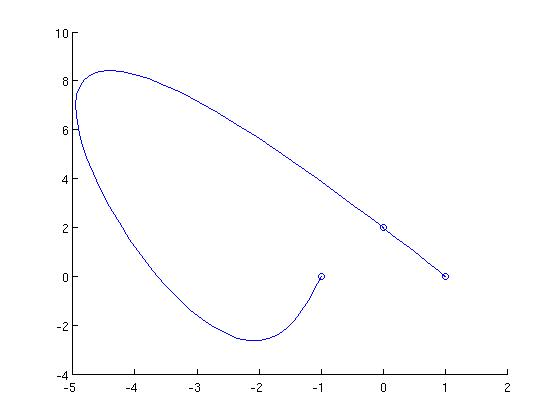
\includegraphics[scale=0.5]{septicspline.jpg}
\caption{The plot of the septic spline}
\end{figure}

\item[d.] Name one advantage and one disadvantage of choosing a lower order polynomial over a higher one.  

The advantage is you get smoother or more continuious trajectories. For instance you will have much smoother transitions in jerk for quintic splines compared
 to cubic splines. However, higher order splines are also more wild in terms of their path length. As seen above, higher order polynomials can go on much
 wider swinging paths. If you need to stick closely to some points, the higer order you go the less you will maintain closeness.
 
\end{enumerate}

\paragraph{3.}

Calculate the angular velocities $\omega^s$ and $\omega^b$ for the rotation:
\begin{align}
R = e^{\hat{\omega}_1 t} e^{\hat{\omega}_2 t}
\end{align}

\begin{align*}
               R = &\;  e^{\hat{\omega}_1 t} e^{\hat{\omega}_2 t} \\
\implies \dot{R} = &\; \frac{d}{dt}(e^{\hat{\omega}_1 t} e^{\hat{\omega}_2 t}) \\
  = &\; \frac{d}{dt}(e^{\hat{\omega}_1 t}) e^{\hat{\omega}_2 t} + e^{\hat{\omega}_1 t} \frac{d}{dt}(e^{\hat{\omega}_2 t}) \\
  = &\; \hat{\omega}_1 e^{\hat{\omega}_1 t} e^{\hat{\omega}_2 t} + e^{\hat{\omega}_1 t} \hat{\omega}_2 e^{\hat{\omega}_2 t} \\
  = &\; \hat{\omega}_1 e^{\hat{\omega}_1 t} e^{\hat{\omega}_2 t} + e^{\hat{\omega}_1 t} e^{\hat{\omega}_2 t} \hat{\omega}_2 \\
 \dot{R^\top R} =&\;  \dot{R}^\top R + R^\top \dot{R} = 0 \\
\implies \dot{R}^\top R =&\;  - (\dot{R}^\top R)^\top \\
  =&\;  - (\left(\hat{\omega}_1 e^{\hat{\omega}_1 t} e^{\hat{\omega}_2 t} + e^{\hat{\omega}_1 t} e^{\hat{\omega}_2 t} \hat{\omega}_2\right)^\top e^{\hat{\omega}_1 t} e^{\hat{\omega}_2 t})^\top
\end{align*}




\paragraph{4.} 
What skew-symmetric matrix $\hat{\omega} \in so(3)$ corresponds to the rotation
\begin{equation*}
R= \begin{bmatrix}
   -0.3038 &  -0.6313 & -0.7135\\
   -0.9332  &  0.3481   & 0.0893\\
    0.1920   & 0.6930 &  -0.6949\\
\end{bmatrix}
\end{equation*}


Is it unique?

%\bibliography{ref}
%\bibliographystyle{plain}

\end{document}
